% Options for packages loaded elsewhere
\PassOptionsToPackage{unicode}{hyperref}
\PassOptionsToPackage{hyphens}{url}
%
\documentclass[
  ignorenonframetext,
]{beamer}
\usepackage{pgfpages}
\setbeamertemplate{caption}[numbered]
\setbeamertemplate{caption label separator}{: }
\setbeamercolor{caption name}{fg=normal text.fg}
\beamertemplatenavigationsymbolsempty
% Prevent slide breaks in the middle of a paragraph
\widowpenalties 1 10000
\raggedbottom
\setbeamertemplate{part page}{
  \centering
  \begin{beamercolorbox}[sep=16pt,center]{part title}
    \usebeamerfont{part title}\insertpart\par
  \end{beamercolorbox}
}
\setbeamertemplate{section page}{
  \centering
  \begin{beamercolorbox}[sep=12pt,center]{part title}
    \usebeamerfont{section title}\insertsection\par
  \end{beamercolorbox}
}
\setbeamertemplate{subsection page}{
  \centering
  \begin{beamercolorbox}[sep=8pt,center]{part title}
    \usebeamerfont{subsection title}\insertsubsection\par
  \end{beamercolorbox}
}
\AtBeginPart{
  \frame{\partpage}
}
\AtBeginSection{
  \ifbibliography
  \else
    \frame{\sectionpage}
  \fi
}
\AtBeginSubsection{
  \frame{\subsectionpage}
}
\usepackage{amsmath,amssymb}
\usepackage{lmodern}
\usepackage{ifxetex,ifluatex}
\ifnum 0\ifxetex 1\fi\ifluatex 1\fi=0 % if pdftex
  \usepackage[T1]{fontenc}
  \usepackage[utf8]{inputenc}
  \usepackage{textcomp} % provide euro and other symbols
\else % if luatex or xetex
  \usepackage{unicode-math}
  \defaultfontfeatures{Scale=MatchLowercase}
  \defaultfontfeatures[\rmfamily]{Ligatures=TeX,Scale=1}
  \setmainfont[BoldFont = SF Pro Rounded Semibold]{SF Pro Rounded}
  \setmathfont[]{STIX Two Math}
\fi
\usefonttheme{serif} % use mainfont rather than sansfont for slide text
% Use upquote if available, for straight quotes in verbatim environments
\IfFileExists{upquote.sty}{\usepackage{upquote}}{}
\IfFileExists{microtype.sty}{% use microtype if available
  \usepackage[]{microtype}
  \UseMicrotypeSet[protrusion]{basicmath} % disable protrusion for tt fonts
}{}
\makeatletter
\@ifundefined{KOMAClassName}{% if non-KOMA class
  \IfFileExists{parskip.sty}{%
    \usepackage{parskip}
  }{% else
    \setlength{\parindent}{0pt}
    \setlength{\parskip}{6pt plus 2pt minus 1pt}}
}{% if KOMA class
  \KOMAoptions{parskip=half}}
\makeatother
\usepackage{xcolor}
\IfFileExists{xurl.sty}{\usepackage{xurl}}{} % add URL line breaks if available
\IfFileExists{bookmark.sty}{\usepackage{bookmark}}{\usepackage{hyperref}}
\hypersetup{
  pdftitle={444 Lecture 1.1 - Course Overview},
  pdfauthor={Brian Weatherson},
  hidelinks,
  pdfcreator={LaTeX via pandoc}}
\urlstyle{same} % disable monospaced font for URLs
\newif\ifbibliography
\usepackage{graphicx}
\makeatletter
\def\maxwidth{\ifdim\Gin@nat@width>\linewidth\linewidth\else\Gin@nat@width\fi}
\def\maxheight{\ifdim\Gin@nat@height>\textheight\textheight\else\Gin@nat@height\fi}
\makeatother
% Scale images if necessary, so that they will not overflow the page
% margins by default, and it is still possible to overwrite the defaults
% using explicit options in \includegraphics[width, height, ...]{}
\setkeys{Gin}{width=\maxwidth,height=\maxheight,keepaspectratio}
% Set default figure placement to htbp
\makeatletter
\def\fps@figure{htbp}
\makeatother
\setlength{\emergencystretch}{3em} % prevent overfull lines
\providecommand{\tightlist}{%
  \setlength{\itemsep}{0pt}\setlength{\parskip}{0pt}}
\setcounter{secnumdepth}{-\maxdimen} % remove section numbering
\let\Tiny=\tiny

 \setbeamertemplate{navigation symbols}{} 

% \usetheme{Madrid}
 \usetheme[numbering=none, progressbar=foot]{metropolis}
 \usecolortheme{wolverine}
 \usepackage{color}
 \usepackage{MnSymbol}
% \usepackage{movie15}

\usepackage{amssymb}% http://ctan.org/pkg/amssymb
\usepackage{pifont}% http://ctan.org/pkg/pifont
\newcommand{\cmark}{\ding{51}}%
\newcommand{\xmark}{\ding{55}}%

\DeclareSymbolFont{symbolsC}{U}{txsyc}{m}{n}
\DeclareMathSymbol{\boxright}{\mathrel}{symbolsC}{128}
\DeclareMathAlphabet{\mathpzc}{OT1}{pzc}{m}{it}

\setlength{\parskip}{1ex plus 0.5ex minus 0.2ex}

\AtBeginSection[]
{
\begin{frame}
	\Huge{\color{darkblue} \insertsection}
\end{frame}
}

\renewenvironment*{quote}	
	{\list{}{\rightmargin   \leftmargin} \item } 	
	{\endlist }

\definecolor{darkgreen}{rgb}{0,0.7,0}
\definecolor{darkblue}{rgb}{0,0,0.8}

\usepackage[italic]{mathastext}
\usepackage{nicefrac}
\usepackage{istgame}

\setbeamertemplate{caption}{\raggedright\insertcaption}

%\def\toprule{}
%\def\bottomrule{}
%\def\midrule{}
\usepackage{etoolbox}
\AfterEndEnvironment{description}{\vspace{9pt}}
\AfterEndEnvironment{oltableau}{\vspace{9pt}}
\BeforeBeginEnvironment{oltableau}{\vspace{9pt}}
\AfterEndEnvironment{center}{\vspace{9pt}}
\BeforeBeginEnvironment{tabular}{\vspace{9pt}}
\AfterEndEnvironment{longtable}{\vspace{-6pt}}
\ifluatex
  \usepackage{selnolig}  % disable illegal ligatures
\fi

\title{444 Lecture 1.1 - Course Overview}
\author{Brian Weatherson}
\date{}

\begin{document}
\frame{\titlepage}

\begin{frame}{Plan}
\protect\hypertarget{plan}{}
\begin{itemize}
\tightlist
\item
  To introduce the outlines of the course.
\end{itemize}
\end{frame}

\begin{frame}{Associated Reading}
\protect\hypertarget{associated-reading}{}
Read the syllabus!
\end{frame}

\begin{frame}{Three Parts}
\protect\hypertarget{three-parts}{}
\begin{enumerate}
\tightlist
\item
  Game Theory
\item
  Origins of Unfairness
\item
  Group attitudes
\end{enumerate}
\end{frame}

\begin{frame}
\begin{figure}
\centering
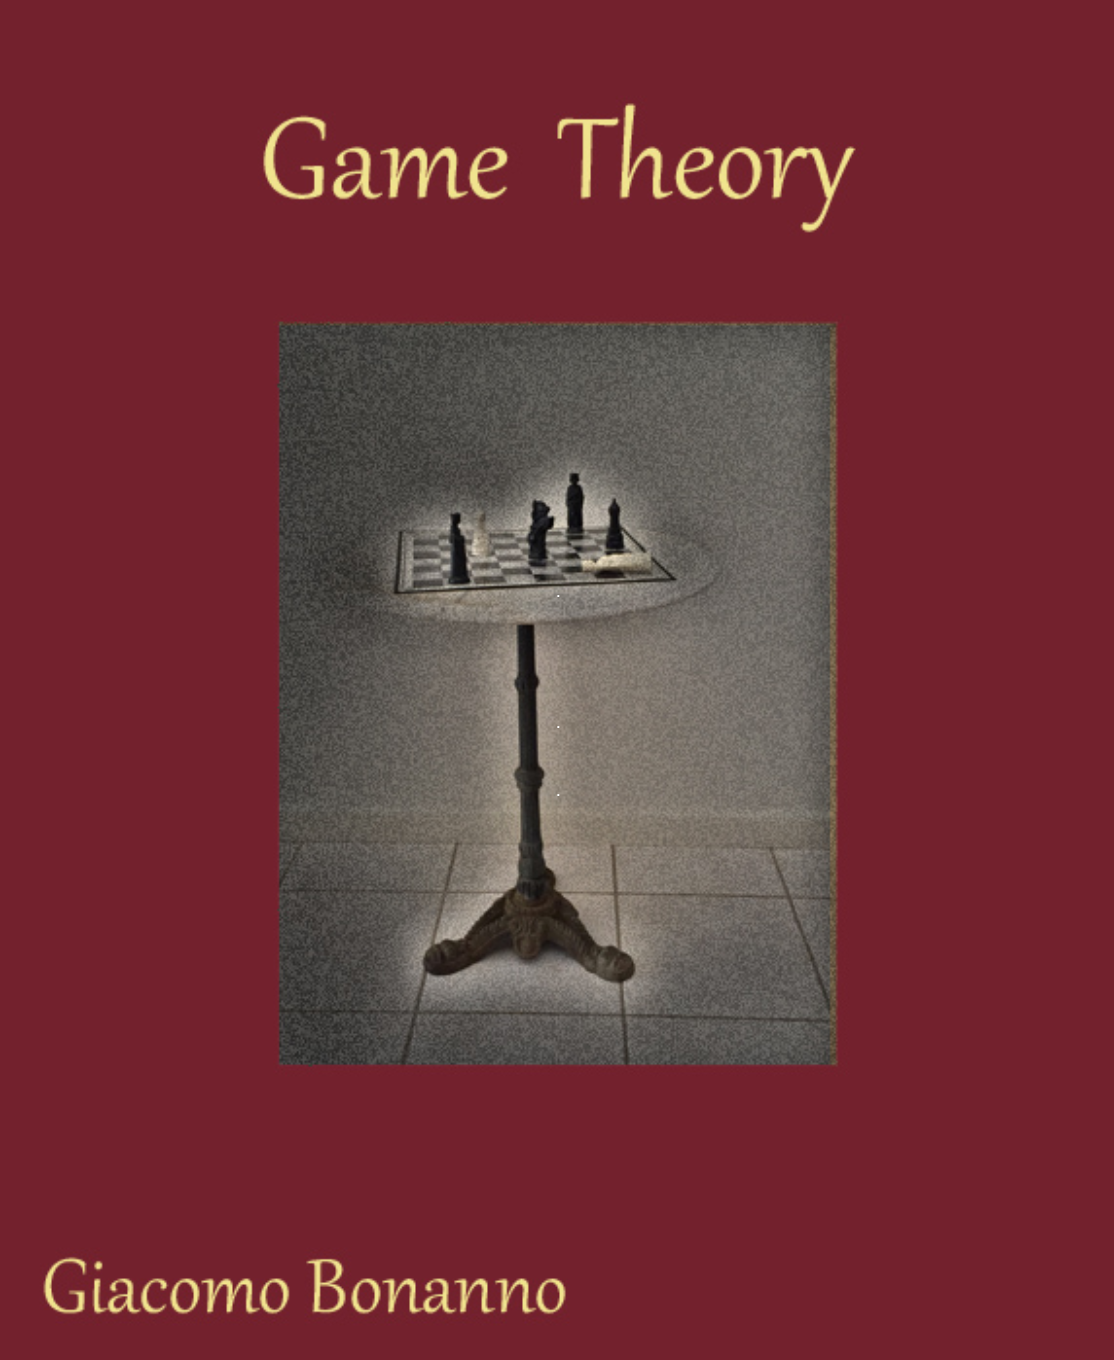
\includegraphics[width=0.65\textwidth,height=0.65\textheight]{images/bonanno_cover.png}
\caption{Giacomo Bonanno, Game Theory}
\end{figure}
\end{frame}

\begin{frame}{Aims}
\protect\hypertarget{aims}{}
\begin{itemize}
\tightlist
\item
  Familiarity with the basic math of game theory.
\item
  Introduce some famous examples of simple game theoretic models that
  get used throughout academic work.
\item
  Look at some attempted explanation of real world phenomena using game
  theoretic tools, and go over the strengths and weaknesses of these
  explanations.
\end{itemize}
\end{frame}

\begin{frame}
\begin{figure}
\centering
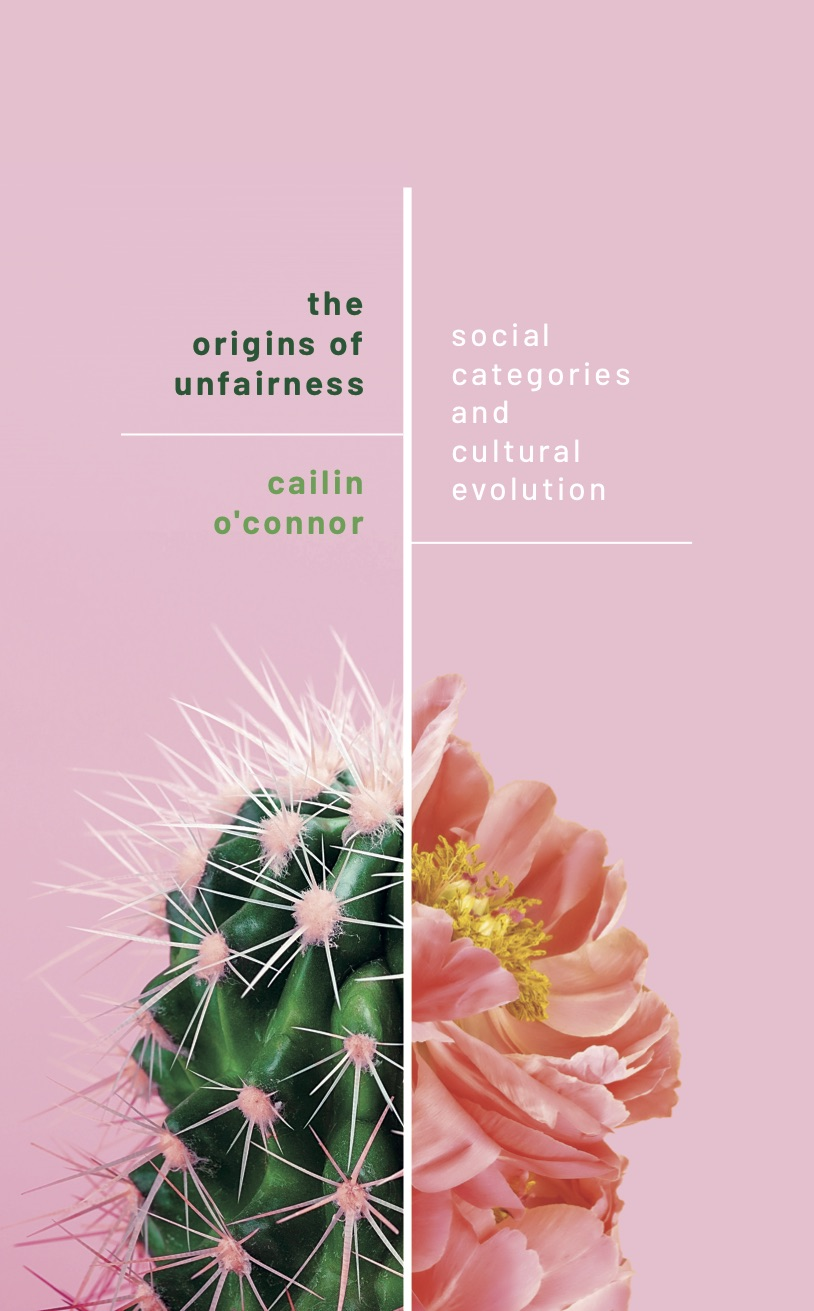
\includegraphics[width=0.65\textwidth,height=0.65\textheight]{images/oconnor_visual.jpg}
\caption{Cailin O'Connor, The Origins of Unfairness}
\end{figure}
\end{frame}

\begin{frame}{Aims}
\protect\hypertarget{aims-1}{}
\begin{itemize}
\tightlist
\item
  Look at game theoretic models of the origin of unequal gender
  distributions.
\item
  Ask whether these models are plausible in light of the facts about how
  this kind of inequality manifests in the real world.
\item
  And in particular, look at the different kinds of gender inequality in
  different parts of life (in particular in workforces vs in households)
  and look at whether the models are as plausible in each case.
\end{itemize}
\end{frame}

\begin{frame}
\begin{figure}
\centering
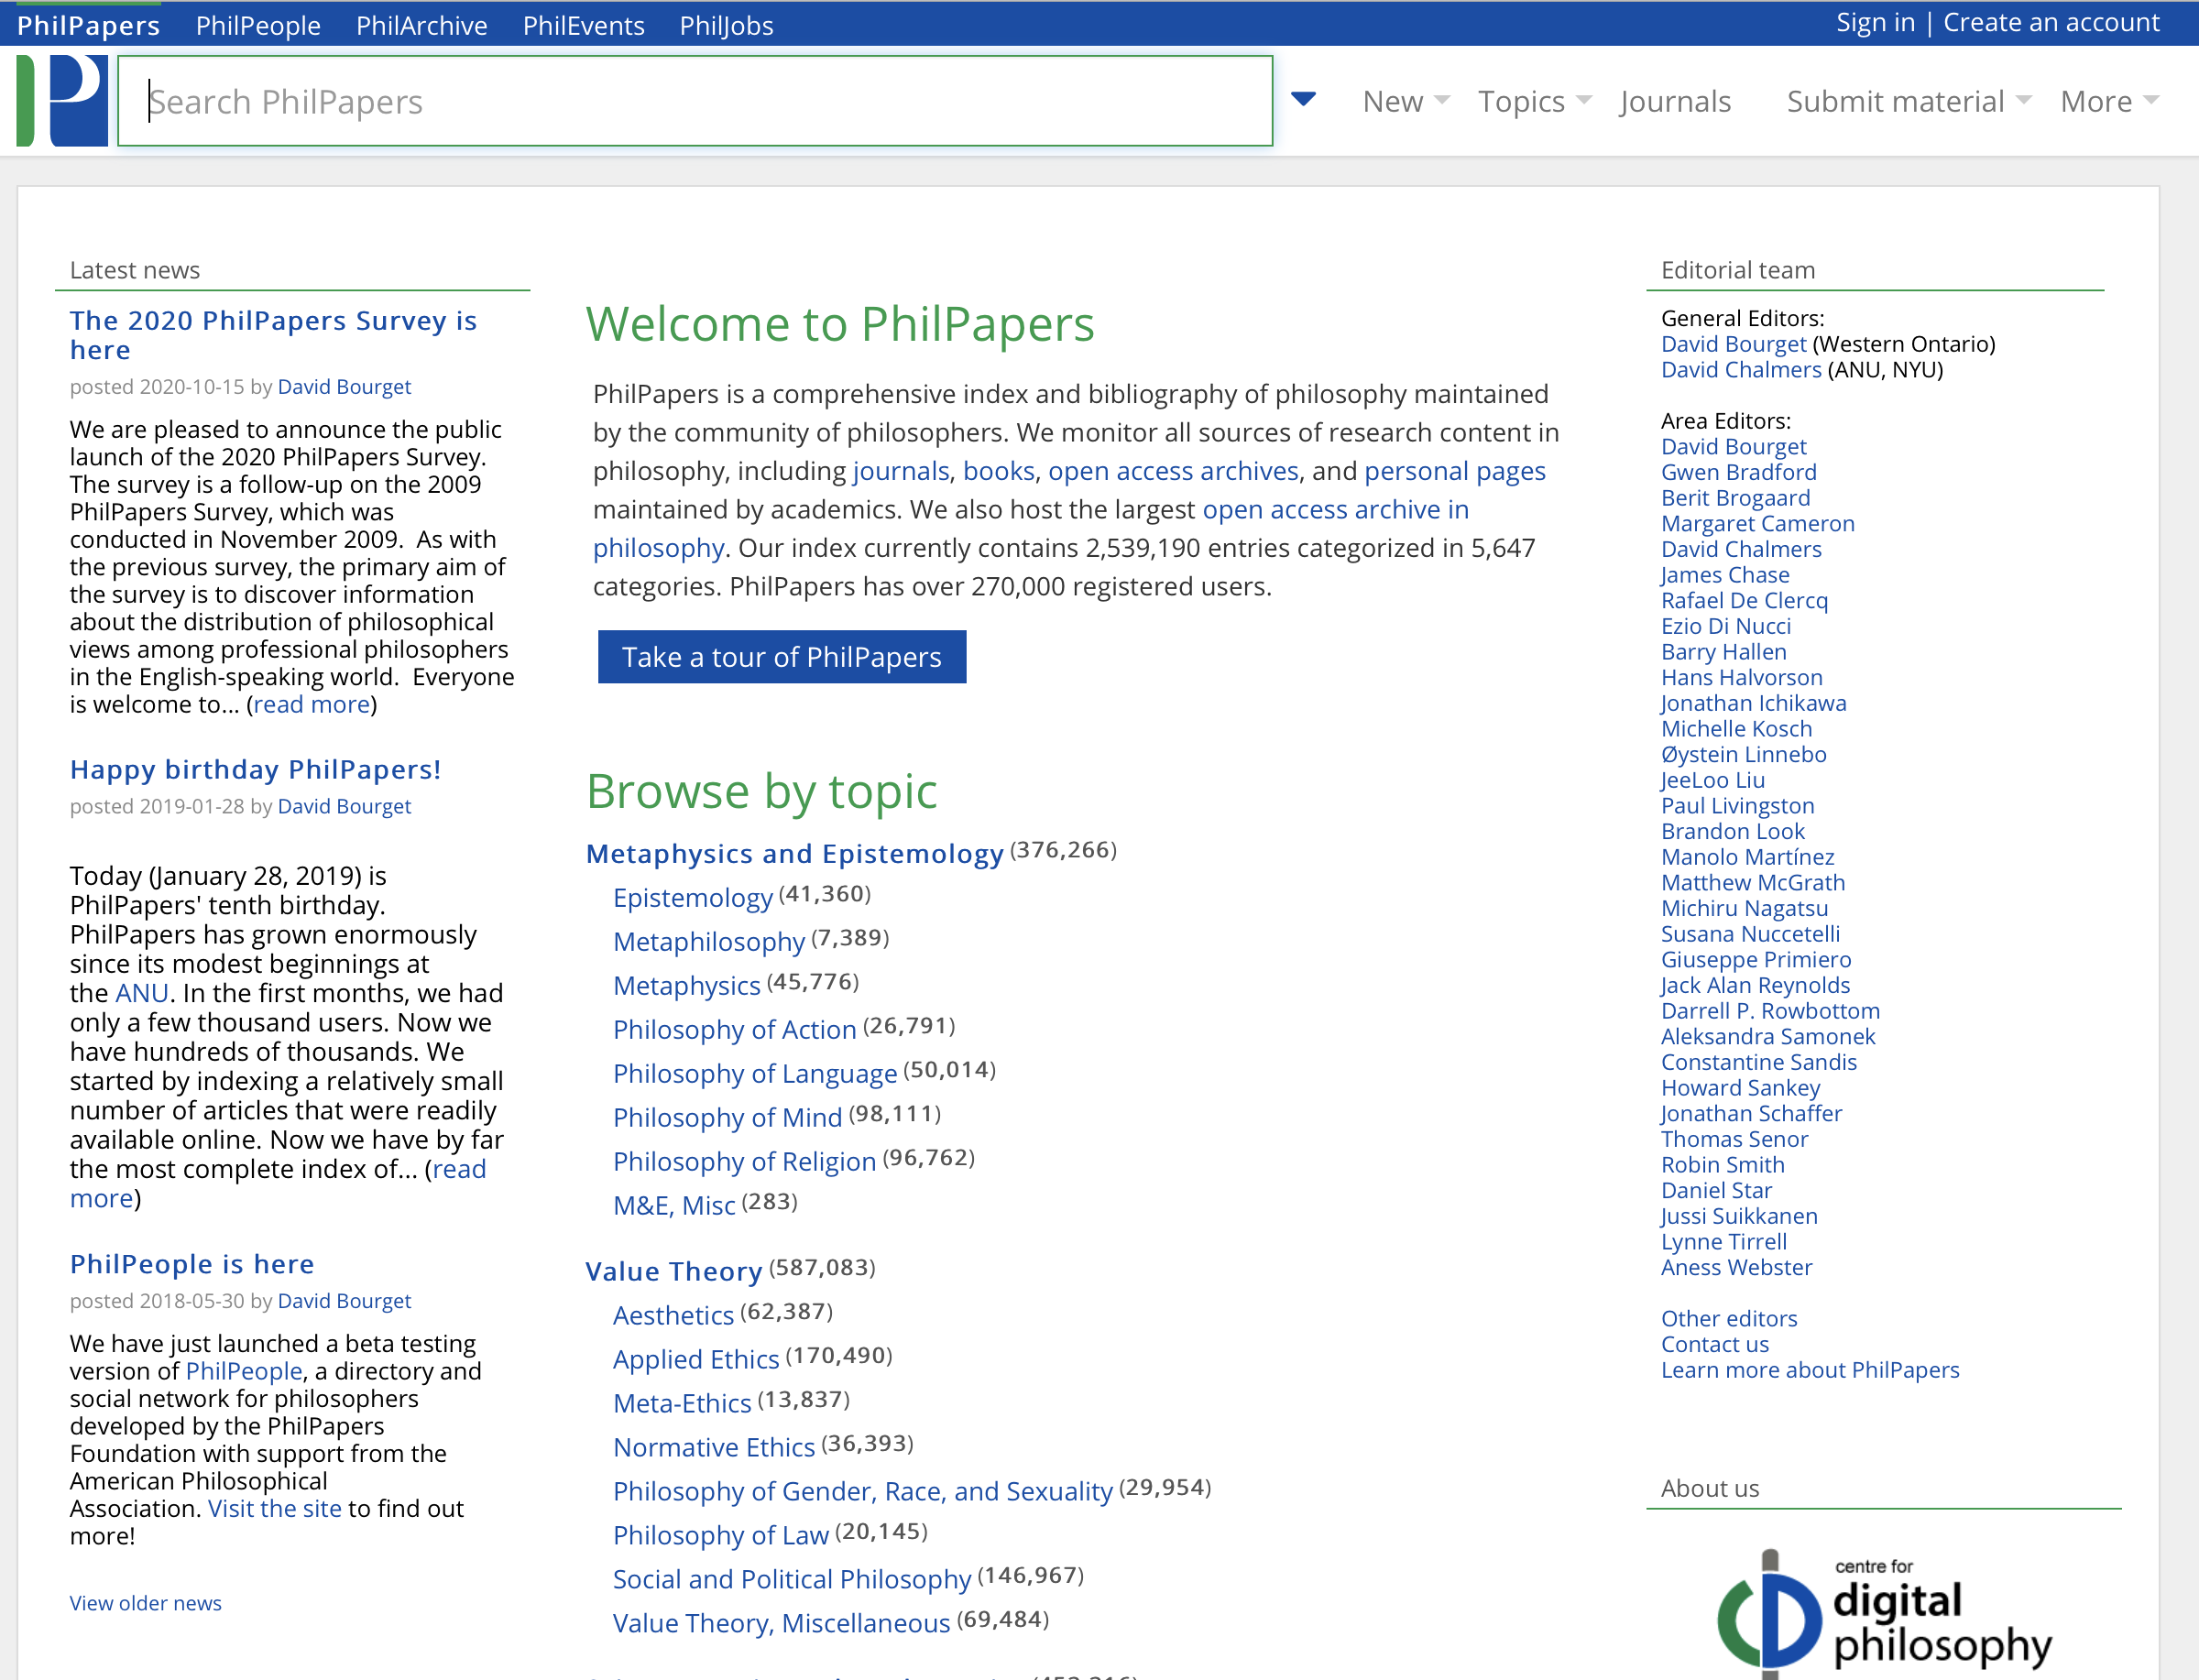
\includegraphics[width=0.65\textwidth,height=0.65\textheight]{images/phil_papers.png}
\caption{PhilPapers}
\end{figure}
\end{frame}

\begin{frame}{Aims}
\protect\hypertarget{aims-2}{}
\begin{itemize}
\tightlist
\item
  Ask whether groups can have attitudes like beliefs, desires, goals,
  intentions, plans and so on.
\item
  Along the way, ask what it means to answer this question positively or
  negatively.
\item
  And, if we have the time, ask what a positive answer would mean for
  our theories of knowledge, responsibility, and so on.
\end{itemize}
\end{frame}

\begin{frame}{Schedule}
\protect\hypertarget{schedule}{}
\begin{itemize}
\tightlist
\item
  Seven weeks on game theory
\item
  Three weeks on unfairness
\item
  Three weeks on group attitudes
\end{itemize}
\end{frame}

\begin{frame}{Schedule Quirk}
\protect\hypertarget{schedule-quirk}{}
\begin{itemize}
\tightlist
\item
  I'm away on January 27, and working around this led to some
  complications with the schedule.
\item
  You'll see things described as `units' not weeks for a little bit on
  the syllabus, because sometimes the material on a Thursday goes best
  with the following Tuesday.
\item
  And for a couple of weeks, the assignments are a little `behind' the
  lectures.
\item
  But we catch up around February 15.
\end{itemize}
\end{frame}

\begin{frame}{Schedule Luck}
\protect\hypertarget{schedule-luck}{}
\begin{itemize}
\tightlist
\item
  The Spring Break falls precisely at the right time for this course;
  just as we switch from the more mathematical part to the more
  discursive part.
\item
  I'd like to claim this was great course design, but it was actually a
  bit of luck.
\end{itemize}
\end{frame}

\begin{frame}{Assessment}
\protect\hypertarget{assessment}{}
\begin{itemize}[<+->]
\tightlist
\item
  Do six small assignments on game theory (the best five will count).
\item
  Write an 8-10 page paper (about 2000 words) on a question from the
  latter two topics
\item
  Each of these will be half of the grade.
\end{itemize}
\end{frame}

\begin{frame}{Week by Week}
\protect\hypertarget{week-by-week}{}
\begin{itemize}[<+->]
\tightlist
\item
  These lectures are recorded ahead of time.
\item
  For the game theory part of the course, they will be the primary part
  of what we do.
\item
  I'll be there for `lectures', but they will just be q\&a, and maybe
  some worked examples. I'm not planning to go 80 minutes each day,
  though I'll stay as long as people have questions.
\item
  Once we get to Part II, I'll still record lecture videos like this
  ahead of time, but they won't go into as much detail.
\item
  There will be discussion sections each week, and they are really
  important.
\end{itemize}
\end{frame}

\begin{frame}{For Next Time}
\protect\hypertarget{for-next-time}{}
\begin{itemize}
\tightlist
\item
  We will start on Bonanno, starting with section 2.1.
\item
  You should also read 2.2 for next Tuesday's class.
\item
  There is no assignment this week, but there will be assignments most
  of the following weeks.
\end{itemize}
\end{frame}

\end{document}
